% Target ~30 pages max: ~10 intro, ~10 methods, ~10 results.
\documentclass[12pt,a4paper,oneside]{report}

\usepackage[T1]{fontenc}
\usepackage[utf8]{inputenc}
\usepackage{lmodern}
\usepackage[british]{babel}
\usepackage[a4paper,margin=2.5cm]{geometry}
\usepackage{setspace}
\onehalfspacing
\usepackage[skip=0.6\baselineskip]{parskip}
\usepackage{microtype}
\usepackage{amsmath,amssymb}
\usepackage{graphicx}
\graphicspath{{figures/}}
\usepackage{float}
\floatplacement{figure}{H}
\usepackage{booktabs}
\usepackage[hyphens]{url}
\usepackage[dvipsnames]{xcolor}
\usepackage{siunitx}
\usepackage{fancyhdr}
\usepackage{titlesec}
\usepackage{caption}
\usepackage[minted,skins]{tcolorbox}
\usepackage{keepsections}
\usepackage{csquotes}

\definecolor{accent}{HTML}{1F4E79}
\definecolor{codebg}{HTML}{F6F8FA}
\definecolor{codeframe}{HTML}{D0D7DE}
\definecolor{figframe}{HTML}{2B80BE}

\newcommand{\thesisimage}[2][]{%
  {\setlength{\fboxsep}{0pt}%
   \setlength{\fboxrule}{1pt}%
   \fcolorbox{figframe}{white}{\includegraphics[#1]{#2}}}%
}

\DeclareCaptionLabelSeparator{pipe}{\ \textcolor{accent}{\textbar}\ }
\captionsetup{font=small,labelfont={bf,color=accent},labelsep=pipe,justification=centering}

\titleformat{\chapter}[block]
  {\normalfont\huge\bfseries}
  {\textcolor{accent}{\thechapter}\hspace{0.5em}\textcolor{accent!40}{\vrule width 1.5pt}\hspace{0.5em}}{0pt}{}
  [\vspace{4pt}{\color{accent!40}\titlerule[0.8pt]}]
\titleformat{name=\chapter,numberless}[block]
  {\normalfont\huge\bfseries}{}{0pt}{}
  [\vspace{4pt}{\color{accent!40}\titlerule[0.8pt]}]
\titlespacing*{\chapter}{0pt}{0pt}{1.5em}
\titleformat{\section}{\normalfont\Large\bfseries}{\textcolor{accent}{\thesection}}{0.8em}{}
\titleformat{\subsection}{\normalfont\large\bfseries}{\textcolor{accent}{\thesubsection}}{0.8em}{}
\titlespacing*{\section}{0pt}{1.2em}{0.4em}
\titlespacing*{\subsection}{0pt}{1em}{0.3em}

\setminted{fontsize=\small,breaklines,autogobble,style=friendly}
\newtcblisting{code}[2][]{
  listing engine=minted, minted language=#2, listing only,
  enhanced, colback=codebg, colframe=codeframe, boxrule=0.5pt, arc=3pt,
  left=6pt, right=6pt, top=2pt, bottom=2pt,
  borderline west={2.5pt}{0pt}{accent}, #1
}

\usepackage[style=apa,backend=biber]{biblatex}
\addbibresource{references.bib}

\usepackage{hyperref}
\hypersetup{colorlinks, linkcolor=accent, citecolor=accent, urlcolor=accent}
\usepackage[capitalise,noabbrev]{cleveref}

\pagestyle{fancy}
\fancyhf{}
\fancyhead[L]{\small\color{gray}\nouppercase{\leftmark}}
\fancyhead[R]{\small\color{gray}\nouppercase{\rightmark}}
\fancyfoot[C]{\thepage}
\renewcommand{\headrulewidth}{0.4pt}
\renewcommand{\headrule}{{\color{accent!30}\hrule height\headrulewidth}}
\setlength{\headheight}{15pt}
\fancypagestyle{plain}{\fancyhf{}\fancyfoot[C]{\thepage}\renewcommand{\headrulewidth}{0pt}}

\newcommand{\todo}[1]{\colorbox{red!10}{\textcolor{red!70!black}{\textbf{TODO:} #1}}}

\newcommand{\thesistitle}{Accelerating and Generalising the Numerical Simulation of Stimulated Brillouin Scattering Dynamics}
\newcommand{\thesisauthor}{Jensen Jones}
\newcommand{\studentid}{24935900}
\newcommand{\thesisdegree}{Bachelor of Computing Science (Honours)}
\newcommand{\supervisors}{%
  \supervisor{Christopher Poulton}{School of Mathematical and Physical Sciences, University of Technology Sydney}%
  \supervisor{Michael Steel}{School of Mathematical and Physical Sciences, Macquarie University}%
}

\hypersetup{pdftitle={\thesistitle}, pdfauthor={\thesisauthor}}

\begin{document}

\pagenumbering{alph}
\begin{titlepage}
  \centering
  \setlength{\parskip}{0pt}
  \vspace*{\stretch{1}}
  {\LARGE\bfseries\color{accent} \thesistitle\par}
  \vspace{1.5em}
  {\color{accent!40}\rule{0.4\textwidth}{0.8pt}\par}
  \vspace{1.5em}
  {\Large \thesisauthor\par}
  \vspace{0.3em}
  {\large Student ID: \studentid\par}
  \vspace*{\stretch{1}}
  \vspace{0.5em}
  {\large\itshape \thesisdegree\par}
  \vspace*{\stretch{1}}
  {\large\bfseries Supervisors\par}
  \vspace{0.6em}
  \newcommand{\supervisor}[2]{{\large #1\par}{\small\itshape #2\par}\vspace{0.6em}}
  \supervisors
  \vspace*{\stretch{1.5}}
  {\large Faculty of Engineering and Information Technology\\ University of Technology Sydney\par}
  \vspace{0.8em}
  {\large November 2026\par}
\end{titlepage}


\pagenumbering{roman}
\chapter*{Abstract}
\addcontentsline{toc}{chapter}{Abstract}

Stimulated Brillouin Scattering (SBS) is an interesting effect in nonlinear optics with applications in lasers, sensing, and signal processing.
Modelling SBS requires solving a set of coupled nonlinear partial differential equations, and analytic solutions
exist only for the most trivial of cases. To accurately model SBS for non-trivial research questions, numerical simulation is required.
This research extends an existing C++ codebase for SBS simulation, started by Professor Michael Steel in November 2025,
to test how the simulation can be improved in performance, through GPU acceleration, and in usability for physicists.

Work on this project began by adding the ability for custom functions to be defined in a simple arithmetic language, in one central
location, which can then be altered by physicists for their research needs. This means custom functions for pulse shapes or spatially
dependent coupling fields can be added without making any code changes. From there, the class \texttt{FieldData} was introduced
as an abstraction around the hardware location and library used for the underlying data storage, allowing the GPU
to be used for computation in a backwards-compatible manner without regressing the existing CPU performance.
Benchmarking then showed that for sufficiently large workloads, by utilising a GPU for computation, the simulation can run
roughly $19\times$ faster, which represents a substantial performance improvement that can greatly reduce experimentation
turnaround time for physicists.

\tableofcontents
% \listoffigures

\clearpage
\pagenumbering{arabic}

\chapter{Introduction}

\section{Background}

\subsection{What Is Stimulated Brillouin Scattering?}

Stimulated Brillouin Scattering (SBS) is a nonlinear optical effect that occurs due to the interaction between light and sound within a material 
\parencite{eggletonBrillouinScatteringPart2022}. When a strong optical (pump) wave, typically from a laser, travels through a medium, 
it undergoes Brillouin scattering as it interacts with co-propagating acoustic (density) waves generated within the medium through 
changes in density induced by strong electric fields. These acoustic waves form a moving refractive index grating 
that scatters part of the light backwards, producing a backward-propagating, frequency-shifted Stokes wave. 
The interaction between these three waves creates a strong self-reinforcing amplification of the Stokes and acoustic waves, 
which leads to exponential growth of the Stokes wave as energy is progressively drained from the pump.

The Brillouin scattering effect most commonly occurs due to the acoustic waves being optically excited. 
The two main physical effects related to this scattering are as follows: first, acoustic waves compress the medium, which alters 
its optical permittivity via photoelasticity. Second, acoustic waves deform the physical boundaries of the medium, which directly 
alters the permittivity at its edges and interfaces.

\begin{figure}
  \centering
  \thesisimage[width=0.85\textwidth]{SBS-picture-with-the-levels}
  \caption{Pump and Stokes wave interaction through time \parencite{baiStimulatedBrillouinScattering2018}.}
  \label{fig:SBSWithLevels}
\end{figure}

A key result of this scattering effect is that the backward-propagating Stokes wave is frequency-shifted relative to the pump. 
This is known as the Brillouin Frequency Shift (BFS). It arises because the acoustic waves (acting as an acoustic grating) are moving, 
so the scattered light experiences a Doppler shift and momentum change. In silica fibre at a wavelength of \qty{1550}{\nano\metre}, 
this downshift is typically around \qty{11}{\giga\hertz} \parencite{agrawalNonlinearFiberOptics2019}. The pump, the acoustic wave and 
the Stokes wave therefore form a feedback loop, and it is this self-reinforcing amplification that the \enquote{stimulated} in SBS refers to.

\subsection{Applications of SBS}

SBS has many important applications in modern photonics and can act as both a useful tool and a limiting constraint in systems 
\parencite{baiStimulatedBrillouinScattering2018}.

In optical signal processing, SBS can help create narrow-linewidth fibre lasers and amplifiers, which are essential for 
high-precision sensing and signal processing in systems where narrow linewidths are important for signal coherence and 
minimising noise \parencite{agrawalNonlinearFiberOptics2019}. Another important application is detecting changes in the 
environment such as temperature and pressure. This capability makes SBS useful for distributed sensing, such as monitoring the 
structural health of civil infrastructure. The main approach for such sensing is known as Brillouin Optical Time Domain Analysis.

Brillouin scattering can also have a negative effect on optical systems. 
Backscattering can occur due to SBS in high-power fibre optic systems, limiting the peak power that can be transmitted without 
distortion or noise. These effects increase with propagation distance, leading to further distortion. Furthermore, in high-power 
fibre lasers and amplifiers SBS acts as the dominant effect that caps the output power. This happens once the pump exceeds the SBS 
threshold and energy is redirected into the backward-propagating Stokes wave rather than the intended output.

Whether trying to suppress or use SBS, accurate simulation of its dynamics is important for understanding the effects 
within a system. These effects rarely have analytic solutions, thus motivating the need for a generalised simulation framework.

\subsection{The Main Equations of SBS}

SBS dynamics are governed by the three-wave interaction equations, \cref{eq:sbs}:
\begin{subequations}
\label{eq:sbs}
\begin{alignat}{2}
  \left(\frac{\partial}{\partial T} + V_1\frac{\partial}{\partial Z} + \mu_1\right) a_1 &= -\kappa\, a_2 b,  &\qquad& \text{(Pump)} \label{eq:pump}\\
  \left(\frac{\partial}{\partial T} + V_2\frac{\partial}{\partial Z} + \mu_2\right) a_2 &= \kappa\, a_1 b^*, && \text{(Stokes)} \label{eq:stokes}\\
  \left(\frac{\partial}{\partial T} + V_3\frac{\partial}{\partial Z} + \mu_3\right) b   &= \kappa\, a_1 a_2^*. && \text{(Acoustic)} \label{eq:acoustic}
\end{alignat}
\end{subequations}

These equations are a system of coupled, nonlinear partial differential equations, which describe the evolution of the three main 
wave envelopes. 
Here $a_1$, $a_2$ and $b$ are the slowly varying envelopes of the pump, Stokes and acoustic fields respectively. 
They are functions of position $Z$ along the waveguide and time $T$. $V_1$, $V_2$ and $V_3$ are the velocities at which each envelope 
travels along the waveguide, $\mu_1$, $\mu_2$ and $\mu_3$ are the corresponding linear damping rates, and $\kappa$ is the 
coupling coefficient that sets the strength of the interaction between the waves. The asterisk denotes the complex conjugate. 

Each equation shares the same structure, where the left-hand side contains a time derivative, a spatial derivative scaled by the 
respective wave's velocity, and a linear damping term. The right-hand side captures the nonlinear coupling between the three waves through the coupling coefficient $\kappa$. Energy from the pump is drained by the Stokes 
and acoustic waves, hence the right-hand side of \cref{eq:pump} carries a negative sign. These equations represent a simplified three-wave 
model that neglects the optical Kerr effect and acoustic noise, to isolate the core dynamics of SBS 
\parencite{montesThreeWaveDissipativeBrillouin2008}.

\Cref{fig:PulseSimulated} illustrates the kind of result sought: given the envelopes at the start, the simulation evolves them 
to give their values at later times.

\begin{figure}
  \centering
  \thesisimage[width=0.85\textwidth]{SimpleGaussianProp}
  \caption{A Gaussian pulse before (left) and after (right) linear propagation. Solid lines show the envelope amplitude 
and dashed lines show its phase. The simulation takes the initial state as input and computes the evolved state.}
  \label{fig:PulseSimulated}
\end{figure}

Numerical simulation of SBS dynamics can be set up in two ways: following how the waves change in space as time passes, or following 
how they change in time as they travel along the waveguide. The equations here use the first. They describe how the shape of each wave 
along the waveguide changes through time. This is the more natural choice for the short structures considered here, where light 
enters and leaves through the ends, because the state of the whole waveguide can be described at one instant and stepped forward in 
time (\cref{fig:PulseSimulated}).

\section{Why Simulation Is Required}

Accurately modelling SBS requires solving a set of coupled nonlinear partial differential equations which define the characteristics 
of the waves. Analytical solutions exist only for simplified cases, such as steady-state operation, where the waves do not change over 
time \parencite{agrawalNonlinearFiberOptics2019}. Once the pump is pulsed or additional effects such as the optical Kerr nonlinearity 
are included, the nonlinear coupling terms in \cref{eq:pump,eq:stokes,eq:acoustic} prevent the equations from being decoupled, and no 
general closed-form solution is known. These cases therefore require numerical simulation.

Numerical simulation overcomes these limitations by providing access to the entire evolution of all three wave envelopes, 
including quantities that are difficult or impossible to measure inside a physical waveguide. It also allows parameters to be varied 
freely and cheaply, enabling researchers to explore system designs, test suppression strategies or sensing configurations, and compare 
theory against experiment before committing to costly fabrication or measurement. The closed-form solutions that do exist for specific 
setups also provide a practical means of testing and validating the simulation's numerical accuracy.


\section{The Existing C++ Codebase}

An existing C++ codebase for the numerical simulation of SBS, created in November 2025 by Professor Michael Steel, provides the basis
on which this research builds. This existing codebase builds and runs on Linux, Windows, and macOS, and is written in C++23 for the core
of the simulation, along with some Python scripts for testing and setup.
The core currently consists of about 14,000 lines of C++ across 97 source files, excluding third-party code, and builds on Eigen for linear algebra, FFTW (MKL on Windows) for Fourier transforms, toml++ for reading the control file, and Catch2 for testing.
It simulates how light pulses travel through an optical waveguide and accounts for SBS and Kerr-nonlinear effects.
Plots of these pulses are output at user-defined intervals of the simulation for analysis, and it can simulate many waves, both forward-propagating
and backward-propagating at the same time.

\begin{figure}
  \centering
  \thesisimage[width=0.85\textwidth]{codebase-architecture}
  \caption{Current codebase architecture schematic.}
  \label{fig:codebase-architecture}
\end{figure}


\Cref{fig:codebase-architecture} shows a very high-level overview of the codebase architecture.
A TOML file configures the specifics of the situation. This file can be used to change a variety of aspects of the simulation, including which linear and nonlinear effects are active, the shape of each forward- and backward-propagating pulse (one of three preset shapes), and the analysis settings.
This file is then parsed internally to set up the starting conditions for the simulation in the Parameters and Simulation Context stages.
The simulation supports a user choice of propagation methods which define how the effects are applied to the pulses at each time step.
The chosen solver (propagation method) is used in the Propagation stage for every step of the simulation, and defaults to symmetric split-step if omitted from the configuration file.
Throughout propagation, the pulse may periodically be printed on a separate thread for analysis, then once the propagation finishes, the final analysis is done in the Analysis stage.

Most components in the Parameters and Simulation Context stages are default-constructed and then configured by a separate
\texttt{setup()} call once the parameters they depend on have been parsed.
This two-phase initialisation departs from standard C++ practice, under which
a constructor should leave an object fully initialised and usable
\parencite{CoreGuidelines}. Here, an object is in an unusable state until
\texttt{setup()} has been called. The pattern is nonetheless common in
scientific computing libraries such as PETSc, where objects are created,
configured, and then explicitly set up in separate steps \parencite{UserGuidePETSc3261}.
It allows components to be declared as plain members of the classes that own
them and configured later, in the order their dependencies require.

Physical models of SBS involve quantities spanning many orders of magnitude, such as $10^{-27}\,\mathrm{s^2/m}$, alongside lengths in metres.
Entered directly into a computer, these values risk overflow and underflow, and make it hard to tell whether the behaviour of the simulation is correct.
These differences in scale are only a side effect of the chosen units: rescaling each quantity by a characteristic value, known as non-dimensionalisation, brings them back to similar sizes.
Theorists commonly work this way, while experimentalists generally prefer to work with physical units.
The codebase supports both through the \texttt{solver.normalise\_quantities} option in the TOML file.

\section{Propagation Methods}

The existing SBS simulation has three different propagation methods: symmetric split-step, interaction-picture fourth-order Runge--Kutta (RK4), 
and interaction-picture Cash--Karp Runge--Kutta (RK5). All three methods solve the same coupled slowly varying envelope equations but differ 
in how they apply the linear and nonlinear effects.
Writing the linear and nonlinear operators as $\mathcal{D}$ and $\mathcal{N}$, advancing the field over a step $h$ is equivalent to
applying $e^{h(\mathcal{D}+\mathcal{N})}$. The operators stay the same throughout the simulation, and only the field is updated at each step. On the numerical grid these operators become matrices that do not commute, so
$e^{h\mathcal{D}}e^{h\mathcal{N}} \neq e^{h(\mathcal{D}+\mathcal{N})}$, but the two become very close when $h$ is small, which is why the
methods take many short steps.

The symmetric split-step method advances the field from $z_k$ to $z_{k+1}$ by applying a half step ($h_k/2$) 
of linear effects, followed by a full step ($h_k$) of nonlinear effects starting from that result, 
then a second half step of linear effects. \Cref{fig:symmetric-split-step} illustrates the symmetric splitting: 
the red $\mathcal{D}$ arrows represent linear half steps, while the blue $\mathcal{N}$ arrows represent full nonlinear steps, 
and the dashed arrows carry each result to the start of the next operator.
Although the nonlinear step is evaluated using RK4, the overall symmetric split-step method is second-order accurate in time.

\begin{figure}
  \centering
  \thesisimage[width=0.8\textwidth,trim=0 0 30 0,clip]{symmetric-split-step}
  \caption[Symmetric split-step propagation]{Symmetric split-step propagation, with computational step $k$ shown in the dashed box \parencite{balacMathematicalAnalysisAdaptive2014}.}
  \label{fig:symmetric-split-step}
\end{figure}

The RK4 method is fourth-order accurate in time, so halving the time step is expected to reduce the global temporal error by approximately 
a factor of 16. In comparison, the second-order symmetric split-step method reduces its error by approximately a factor of four. 
However, RK4 requires more function evaluations per step, meaning its higher convergence order does not necessarily translate to greater 
computational efficiency.

\begin{equation}
  \label{eq:rk4}
  \begin{aligned}
    A^{(i)} &= U_{h/2}^{\mathcal{D}} A_n, \\
    k_1 &= U_{h/2}^{\mathcal{D}} f(A_n, z_n), \\
    k_2 &= f\!\left(A^{(i)} + \tfrac{h}{2}k_1,\, z_n + \tfrac{h}{2}\right), \\
    k_3 &= f\!\left(A^{(i)} + \tfrac{h}{2}k_2,\, z_n + \tfrac{h}{2}\right), \\
    k_4 &= f\!\left(U_{h/2}^{\mathcal{D}}\left(A^{(i)} + h k_3\right),\, z_n + h\right), \\
    A_{n+1} &= U_{h/2}^{\mathcal{D}}\left[A^{(i)} + \tfrac{h}{6}\left(k_1 + 2k_2 + 2k_3\right)\right] + \tfrac{h}{6}k_4.
  \end{aligned}
\end{equation}

The fourth-order Runge--Kutta method evaluates the nonlinear derivatives at four intermediate stages, which are then combined using a weighted average and applied to the field, as shown in \cref{eq:rk4}. The linear part of the problem is easy: because $\mathcal{D}$ is diagonal in Fourier space, dispersion alone can be solved arbitrarily far ahead in a single step. The nonlinear part cannot be diagonalised and has no such solution except in special cases, so the whole problem cannot be solved in one step. The interaction picture takes advantage of this by instead moving the easy linear part onto the operators, the $U^{\mathcal{D}}_{h} = e^{h\mathcal{D}}$ terms in \cref{eq:rk4}, and leaving only the hard nonlinear part on the field for RK4 to integrate, which reduces the work done per step. Unlike the symmetric split-step method, the RK4 implementation incorporates the linear effects throughout, allowing the interaction between linear and nonlinear effects to be accounted for within each step. This requires four nonlinear derivative evaluations per step, increasing the computational cost per step compared to simpler integration schemes.

Similarly, the RK5 method of propagation is fifth-order accurate in time, so halving the time step reduces the temporal error by approximately a factor of 32. This comes at the cost of additional calculations at each step. \Cref{eq:rk5-stages} in \cref{app:rk5} gives all six stages of the RK5 method, and \cref{eq:rk5-solution} the fifth-order solution built from them. The Cash--Karp scheme also embeds a fourth-order solution built from the same six stages, and the difference between the two provides a local error estimate that can be used to adapt the step size \parencite{balacMathematicalAnalysisAdaptive2014}.


\section{The Research Gap}

The focus of this research project is to improve the simulation software in terms of three main criteria: performance, modularity and portability. Program performance is fundamental for timely running of large simulations and reducing the time spent waiting for results. Improving the modularity of the program means it can be easily extended for further research without compromise, for example by adding a new nonlinear effect in one localised part of the code. Portability is important for the program to not just be able to run on any device but to be able to do so efficiently.

Current approaches to simulation software typically focus on creating instruments useful for either theoretical physicists or experimental physicists, rarely addressing the needs of both. Theoretical research focuses on working with idealised or unattainable conditions, whereas experimental research is constrained by real-world limitations. This research project will address the need to create software that meets the requirements of both sides without compromising on either.

When well-developed libraries for simulation do not exist, the common practice in research is to write ad-hoc Python scripts tailored to a specific experimental configuration, use them once, and discard or abandon them for the next task. While Python allows for rapid prototyping, these scripts accumulate technical debt quickly and consequently are rarely used beyond their original purpose. Python's interpreted nature also restricts the performance of any simulations run. This means that each new research task effectively starts from scratch, with researchers reinventing core SBS simulation logic repeatedly rather than building on a stable foundation.

\section{Research Significance and Physics Outcomes}

The significance of this research lies in producing an enhanced simulation codebase for SBS that can serve as a reusable and extensible foundation for future research. Different research requires different environmental configurations, such as pulse shapes and other nonlinear and linear effects. A flexible and tunable library allows researchers to easily adapt the software to the specific needs of their research, cutting out the time that would be spent rewriting core SBS logic for each specific research task. Well-written and flexible code also means that as new discoveries occur, they can be added to the library without large architectural changes.

From a performance standpoint, the aim of this research project is for all simulations to run faster, leading to less dead time for researchers whilst waiting for results. This outcome is most important for simulations done at a large scale. By writing well-optimised C++ and GPU (graphics processing unit) accelerated code, not only does the code become more efficient for all simulations, but it can also make it practical to simulate conditions that were previously too large to simulate, potentially revealing unseen effects.

To increase the modularity of the system, on top of writing clean C++ that follows best coding practices, the research will add custom function definitions that can be used to define waves and other spatially dependent fields. This will free researchers from a preset set of options and broaden what can be simulated. Clean coding practices also make the library easy to extend for specific research needs.

To address portability, all changes will consider the ability of the codebase to be developed and executed across different 
operating systems (typically macOS or Linux for theorists and Windows for experimentalists).
This will lead to fewer barriers to using and extending the library for all types of physicists.

\section{Research Objectives}

This research is guided by one central objective: to improve the existing SBS modelling codebase into a library that 
balances performance, modularity for further research, and portability. Success against all three metrics will be 
evaluated through benchmarking, portability testing, and architectural and structural code analysis against software 
engineering best practices.

Performance success is defined as a measurable reduction in wall-clock time for the simulation relative to the 
existing baseline implementation, verified through repeated benchmarking under controlled conditions. 
Modularity success is defined as the ability to add new physics logic in a localised code fashion, 
without modifying unrelated parts of the code, verified through architectural review and testing. Portability success is 
defined as the ability to build and run the codebase across macOS, Windows and Linux without any code changes, 
producing outputs that agree to within floating-point tolerance.

\section{CPU and GPU Computing}

A CPU (central processing unit) is a hardware component responsible for executing computing instructions of a 
specific instruction set architecture (ISA), performing computations and modifying architectural state. 
Modern CPUs contain multiple cores, each of which has its own levels of local cache and is capable of independently 
executing instructions. CPUs are designed for high single-core performance and low execution latency. 
To achieve this, they use a wide range of techniques such as SIMD (single instruction, multiple data) instructions, pipelined instruction processing, 
branch prediction, out-of-order execution, and multi-level cache hierarchies \parencite{stokesMachine2006}.

A GPU, however, is a more specialised piece of hardware originally designed for rendering graphics, 
which now sees widespread use in machine learning, high-performance computing and other computationally intensive workloads. 
GPUs are designed for highly parallel computation, containing thousands of arithmetic execution units organised into multiple 
processing groups. Rather than maximising the computational speed of a single thread, GPUs are designed to maximise 
computational throughput by executing large numbers of threads simultaneously. This makes a GPU well suited to large, 
data-parallel operations where the same computation is applied across many elements \parencite{nickollsGPUComputingEra2010}.

A GPU operates on data held in its own local memory, known as Video Random Access Memory (VRAM), which is 
physically separate from the system RAM used by the CPU. Data produced on one device and needed by the other must 
therefore be copied between the two memories over the interconnect that links them, typically a PCIe bus. 
As illustrated in \cref{fig:gpu-cpu-architecture}, each transfer introduces latency on the order of microseconds, 
and the available bandwidth is limited to approximately \qty{25}{\giga\byte\per\second} for a PCIe~4.0~x16 connection, 
considerably lower than the bandwidth of the GPU's own memory. The total transfer time therefore depends on both 
the fixed overhead per transfer and the amount of data being transferred, so workloads that frequently move data 
between the CPU and GPU can lose much of the benefit of GPU acceleration.

\begin{figure}
  \centering
  \thesisimage[width=0.75\textwidth]{gpu-cpu-architecture}
  \caption{High-level GPU and CPU architecture.}
  \label{fig:gpu-cpu-architecture}
\end{figure}

% Plan (~10 pages): 2 custom functions, 4 LibTorch, 1 benchmarking.
\chapter{Methodology}

% Plan: ~2 pages.
\section{Custom Function Support}

The first stage of improving the codebase was adding support to interpret and apply custom functions to describe initial pulse shapes and spatially dependent couplings. The core goal of the implementation was for researchers to be able to define a function in the input TOML control file as a plain mathematical expression, which is then interpreted by the program and applied to the specified field with minimal overhead. ExprTk (Expression Toolkit) is a third-party C++ library for interpreting mathematical expressions written as strings into functions.

\Cref{fig:old-pulse-shape} shows the previous declaration of a Gaussian-shaped forward-propagating pulse called \texttt{launch\_f0}. Previously, this pulse was constrained to be in the shape of a Gaussian, super-Gaussian or sech.

\begin{figure}
\begin{code}{toml}
[launch_fields]
channels = [
  { name = "launch_f0", active = true, shape = "gaussian", ... },
]
\end{code}
  \caption{Old pulse shape specification. Limited to "gaussian", "super-gaussian", or "sech"}
  \label{fig:old-pulse-shape}
\end{figure}

These preset wave shapes are still supported and can be chosen without needing to redefine them as custom wave shapes, keeping the TOML file backwards compatible. Custom functions can be added by declaring a function with a name and a definition \texttt{f}. As seen in \cref{fig:custom-functions}, the preset names can still be referenced without being defined (the \texttt{gaussian} shape in pulse \texttt{launch\_f1}), but custom shape functions such as \texttt{handwrittenGaussian} and \texttt{wobblyPulse} can now also be defined and referenced.

\begin{figure}
\begin{code}{toml}
[spatial_functions]
functions = [
  { name = "handwrittenGaussian", f = "P0 := 2.0; w := 8.0; sqrt(P0) * exp(-x^2 / (2 * w^2))" },
  { name = "wobblyPulse", f = "exp(-x^2 / 50) * (1 + 0.5 * cos(x))" },
]

[launch_fields]
channels = [
  { name = "launch_f0", shape = "handwrittenGaussian", ... },
  { name = "launch_f1", shape = "gaussian", ... },
]
\end{code}
  \caption{Custom defined functions.}
  \label{fig:custom-functions}
\end{figure}

Likewise, custom shapes for spatially dependent coupling fields are defined in the same way, then associated with the desired effect in the TOML file, as shown for \texttt{kappa} in \cref{fig:spatial-coupling}.

\begin{figure}
\begin{code}{toml}
[spatial_functions]
functions = [
  { name = "kapgauss0", f = "w0 := 0.005; kap0 := 10.0; kap0 * sech(x / w0)" },
]

[gratings]
kappa = 10 # constant
# kappa = "kapgauss0" # or a spatial profile
\end{code}
  \caption{Spatially dependent coupling with a custom function.}
  \label{fig:spatial-coupling}
\end{figure}

In the code, both preset and custom shapes are held in a \texttt{CustomFunctionStore}, which maps each shape name to a \texttt{SpatialFunction} object (\cref{fig:function-store}). \texttt{SpatialFunction} is an abstract interface with a single \texttt{generate} method that returns the shape evaluated across the spatial grid. The presets (Gaussian, super-Gaussian and sech) and the user-defined ExprTk expressions are all implementations of this interface. A launch field therefore requests its shape by name and does not need to know whether it is a preset or a custom function.

\begin{figure}
\begin{code}{cpp}
class SpatialFunction {
    virtual Eigen::VectorXcd generate(const Eigen::VectorXd& x) const = 0;
};

class CustomFunctionStore {
    std::unordered_map<std::string, std::unique_ptr<SpatialFunction>> nameToSpatialFunction;
public:
    Eigen::VectorXcd generate_spatial_function(const Eigen::VectorXd& x,
                                               const std::string& name) const;
};
\end{code}
  \caption{Simplified structure of the function store.}
  \label{fig:function-store}
\end{figure}

Couplings use the same store, but each value in the control file may be either a constant or the name of a function. It is read as a \texttt{std::variant<double, std::string>} and resolved with \texttt{std::visit}. A number becomes a constant, while a name is looked up in the store and evaluated across the grid. The result is held in a \texttt{SpatiallyDependentCoupling}, which wraps a variant of either a single complex scalar or a complex array and overloads the arithmetic operators. The propagation code can therefore apply a coupling without knowing whether it is uniform or spatially varying, and a uniform coupling remains a single scalar at no extra cost.

Custom functions are parsed by ExprTk once at initialisation and evaluated once per grid point to produce the launch and profile arrays. From then on, the propagation uses ordinary arrays, so flexible user input costs only a one-off setup step and nothing per time step, which is negligible compared with the propagation itself.

% Plan: ~4 pages.
\section{GPU Acceleration with LibTorch}

Adding LibTorch support to the simulation started with how to decide the program should be ran on a GPU.
The chosen approach was for opt-in GPU compute via the configuration TOML.
This can be set by a simple value as seen in \Cref{fig:gpu-opt-in}.

\begin{figure}
\begin{code}{toml}
[general]
compute_backing = "Eigen" # CPU
\end{code}
\begin{code}{toml}
[general]
compute_backing = "LibTorch" # GPU
\end{code}
	\caption{TOML GPU / CPU computation selection.}
	\label{fig:gpu-opt-in}
\end{figure}

This chosen \texttt{compute\_backing} then determines the way that the data is stored internally in the program.
For this, the abstraction of a \texttt{FieldData} object was chosen.
As shown in \Cref{fig:FieldData-code}, \texttt{FieldData} uses a \texttt{std::variant} to hold either an \texttt{EigenFieldData} or a \texttt{TorchFieldData}, 
exposing a common public interface for operations on the underlying data. 
For example, \texttt{fft\_forward\_inplace} applies a forward FFT to each active channel within the first \texttt{ncols} columns.

\begin{figure}
\begin{code}{cpp}
class FieldData {
private:
    std::variant<EigenFieldData, TorchFieldData> impl_;

public:
    void fft_forward_inplace(
        const std::vector<int>& active_channels, long ncols, const FFT_Wrapper& fft_wrapper);

    void assign_exp_scaled_col(long col, dcomplex scale, const FieldData& source);

    ...

}
\end{code}
  \caption{Simplified view of a FieldData}
  \label{fig:FieldData-code}
\end{figure}

This interface decouples the calling code from the underlying storage implementation. 
Consequently, callers can operate on \texttt{FieldData} without needing to know whether the data is backed by Eigen (CPU) or LibTorch (GPU), 
allowing the same code to work with either hardware.

Simplified representations of \texttt{EigenFieldData} and \texttt{TorchFieldData} classes can be seen below in \Cref{fig:BackingSpecificFieldData}

\begin{figure}
\begin{code}{cpp}
class EigenFieldData {
private:
    Eigen::MatrixXcd data_;

public:
    void fft_forward_inplace(const std::vector<int>& active_channels, long ncols, const FFT_Wrapper& fft_wrapper);

    void assign_exp_scaled_col(long col, dcomplex scale, const EigenFieldData& source);

    ...
}

class TorchFieldData {
private:
    torch::Device device_;
    torch::Tensor data_; // shape [rows, cols], complex double or complex float
    
public:
    void fft_forward_inplace(const std::vector<int>& active_channels, long ncols, const FFT_Wrapper& fft_wrapper);

    void assign_exp_scaled_col(long col, dcomplex scale, const TorchFieldData& source);
}
\end{code}
\caption{Simplified view of EigenFieldData \& TorchFieldData}
  \label{fig:BackingSpecificFieldData}
\end{figure}

Each backing-specific implementation of \texttt{FieldData} is required to provide an implementation of every function in the public interface. 
Calls made through a \texttt{FieldData} object are then dispatched to the corresponding function of the underlying type held by \texttt{impl\_}, using \texttt{std::visit}.

This dispatch incurs no runtime overhead compared to a direct function call. The alternatives in \texttt{std::variant} are known at compile time, allowing the compiler to generate efficient dispatch code.
Also, because the visitor must be valid for every possible alternative of the variant,
any missing function implementations result in easily diagnosable compile-time errors.

The two backings require their own unique implementations for these functions because they don't share an interface. 
If both LibTorch and Eigen shared an interface, then FieldData could simply be templated on the underlying type of Eigen 
(\texttt{Eigen::MatrixXcd}) or LibTorch (\texttt{torch::Tensor}). However by doing so it would also restrict future backing types to those that also share an interface.

The nature of this FieldData also makes it easy to define new operations on the data. 
Simply declare the function in the interface class \texttt{FieldData}, define the backing-specific implementations, and then use the helper function
\texttt{visit\_matched\_backings} as seen below in \Cref{fig:visit_matched_backings} to do the \texttt{std::visit} dispatch.

\begin{figure}
\begin{code}{cpp}

// Runs `op` on the backings, throwing error for mismatched backing types.
template <typename VariantA, typename Fn, typename... Variants>
decltype(auto) visit_matched_backings(
    const char* opName, Fn&& op, VariantA&& a, Variants&&... rest) {
    if (((a.index() != rest.index()) || ...)) {
        throw std::invalid_argument(std::format("FieldData::{}: backing mismatch", opName));
    }
    return std::visit(
        [&]<typename T>(T& lhs) -> decltype(auto) {
            return op(lhs, std::get<std::decay_t<T>>(rest)...);
        }, a);
}

\end{code}
\caption{Common \texttt{std::visit} helper method}
\label{fig:visit_matched_backings}
\end{figure}

Factoring computation into smaller backing-specific methods requires understanding the trade-off between reusable code and efficient computation.
The Eigen library for CPU computation uses expression templates to delay evaluation of computation until the final assignment rather than creating temporary objects.
It does this by constructing a lightweight expression object whose type represents the computation at compile time, thus eliminating temporary copies and allocation.
Because of this, although creating the \texttt{FieldData} interface as a set of simple, basic functions and operator overloads would reduce logic duplication in the code, it would prevent Eigen from using expression templates and regress CPU performance.
This is because each function must return a \texttt{FieldData}, whose \texttt{std::variant} can only hold a fully evaluated \texttt{EigenFieldData}, so every call would evaluate its result into a temporary.
Hence, the functions in the \texttt{FieldData} interface were kept coarse enough that each can be written as a single Eigen expression, such that Eigen operations don't lose their performance.
GPU operations through LibTorch don't have the same requirements for their code, as LibTorch evaluates each operation eagerly, launching a GPU kernel per operation regardless of how the code is factored.


When a simulation is run with LibTorch as the selected \texttt{compute\_backing}, the setup stage determines what hardware to store LibTorch tensors on.
This requires determining the type of hardware, as well as specific vendor if GPU.
Below \Cref{fig:hardware-detection} shows how this flow works. 
First, the CUDA API checks whether a GPU is available, then the XPU API checks for an Intel GPU; otherwise, the program defaults to the CPU.
\texttt{resolve\_torch\_device} uses a lazy initialised static variable constructed from an immediately invoked lambda.
This means that the lambda is only called the first time the function runs; subsequent calls return the cached device type.

\begin{figure}
\begin{code}{cpp}
torch::DeviceType resolve_torch_device() {
    static const torch::DeviceType device = [] {
        DeviceType d;
        if (cuda::is_available()) { // NVIDIA GPU
            d = kCUDA;
        } else if (xpu::is_available()) { // intel GPU
            d = kXPU;
        } else {
            d = kCPU; // CPU
        }
        g_logger.info(...);
        return d;
    }();
    return device;
}
\end{code}
\caption{\texttt{resolve\_torch\_device} simplified function for choosing the most powerful owned device for LibTorch}
\label{fig:hardware-detection}
\end{figure}

AMD GPUs are not currently supported by this implementation. 
LibTorch can use AMD GPUs through ROCm, but ROCm support depends on a compatible Linux
environment, an AMD GPU and driver supported by the selected ROCm release, and a matching
ROCm-enabled LibTorch build. In theory, PyTorch can expose ROCm devices through its
CUDA-compatible API, which would be detected in the existing function. However, this hasn't
been tested thoroughly.


To add a new \texttt{compute\_backing} type, such as a \texttt{SyclFieldData} or a \texttt{CudaFieldData},
each function of the public \texttt{FieldData} interface would remain unchanged as it already dispatches to the underlying type.
Once the new \texttt{FieldData} is added to the \texttt{std::variant} type of \texttt{impl\_}, any undefined interface functions of the new type will throw compile time errors.
Once all functions are defined, the code will dispatch to the new \texttt{compute\_backing}.
This code makes the simulation codebase very easy to further experiment with different libraries and hardware.

Building of the binary was also designed for cross platform ease of use.
Users can enable/disable LibTorch builds via a flag so that users intending of running on CPU only don't require any GPU libraries.
This way people without a GPU can still build the program and run simulations without needing to download the GPU libraries.


% Plan: ~1 page.
\section{Benchmarking Suite}

To compare performance across compute backings and simulation configurations, I developed a
Python benchmarking suite that runs the simulation over controlled parameter sweeps. The main
runner can be specified to vary a specific attribute of the run such as grid size, compute backing,
propagation method, or the number of optical channels. For each configuration, the suite repeats the
simulation and records its runtime in a CSV file. It captures total simulation time, as well as the time
spent in linear and nonlinear parts of each step. A plotting script then interprets the CSV and visualises the results.
The results generated from this benchmarking suite will be shown in the following chapter on results.

% Plan (~10 pages).
\chapter{Results}

% Plan: ~1 page.
\section{Simulation Outputs}

\Cref{fig:simulation-gaussian-evolution} shows the field amplitude at the start and end of a
simulation with a Gaussian input pulse and group-velocity dispersion enabled. The pulse
broadens during propagation, while its peak amplitude decreases. This is the expected change
for a dispersive pulse and provides a simple example of the field output produced by the
simulation.

\begin{figure}
  \centering
  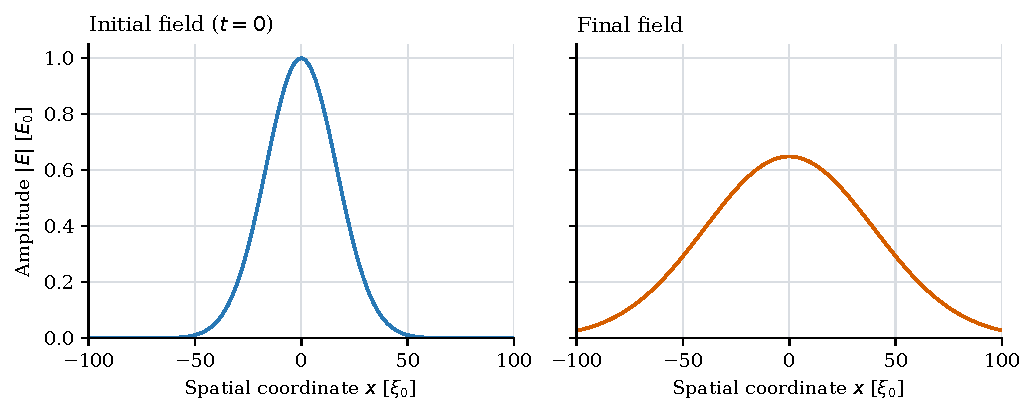
\includegraphics[width=\textwidth]{simulation_gaussian_evolution}
  \caption{Initial and final field amplitudes for the built-in Gaussian channel in a
  group-velocity-dispersion simulation. Both panels show the same spatial range,
  $-100 \leq x/\xi_0 \leq 100$. The final pulse is broader and has a lower peak amplitude.}
  \label{fig:simulation-gaussian-evolution}
\end{figure}

As discussed earlier, the simulation now allows for custom defined pulse shapes. An example
of this can be seen below in \Cref{fig:simulation-builtin-custom} which shoes the pre and post 
simulation of these shapes. For this example, the custom amplitude profile is
\(\exp(-x^2/50)(1 + 0.5\cos(x))\), the same as seen in \Cref{fig:custom-functions}.
The two profiles are launched as separate forward channels in the same simulation,
illustrating that a custom shape can be used alongside a preset shape.

\begin{figure}
  \centering
  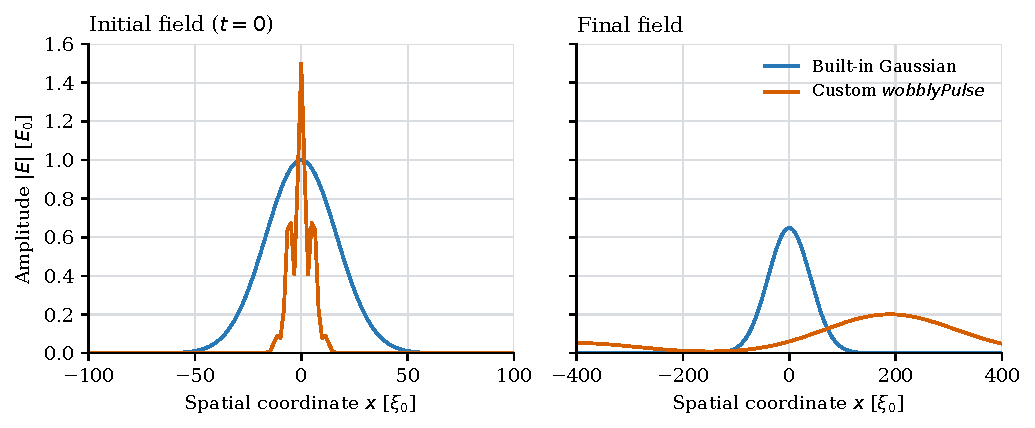
\includegraphics[width=0.9\textwidth]{simulation_builtin_vs_custom}
  \caption{Initial (left) and final (right) field amplitudes for the built-in Gaussian and
  custom pulse, launched as two forward channels in one simulation. The Gaussian's initial
  profile is the same as in \cref{fig:simulation-gaussian-evolution}. The horizontal ranges
  differ to show the full profiles before and after propagation.}
  \label{fig:simulation-builtin-custom}
\end{figure}

% Plan: ~2 pages.
\section{Performance Benchmarking}

The first performance experiments isolated the linear propagation path by disabling all
nonlinear effects. The linear computation was the first part ported to using \texttt{FieldData}
objects, and hence benchmarking acted as a proof of concept. The experiments compared the
Eigen CPU implementation with LibTorch on the GPU while varying the number of spatial grid
points and optical channels.

\Cref{fig:linear-grid-sweep} shows total simulation time for one optical channel as the grid
size increases. At the smallest measured grid size, the GPU was slower than the CPU (a
CPU-to-GPU time ratio of 0.5). The GPU became faster as the problem grew: the ratio reached
6.6 at 131,072 grid points and 18.6 at 1,048,576 grid points. Below grid sizes of $2^{15}$, 
the cost of launching a GPU operation becomes the main cost in time, and the actual operations 
don't become any faster, so the CPU is able to be quicker in those situations. In practice,
grid points would be kept above this level for higher precision, and the GPU advantage would 
be relevant.

\begin{figure}
  \centering
  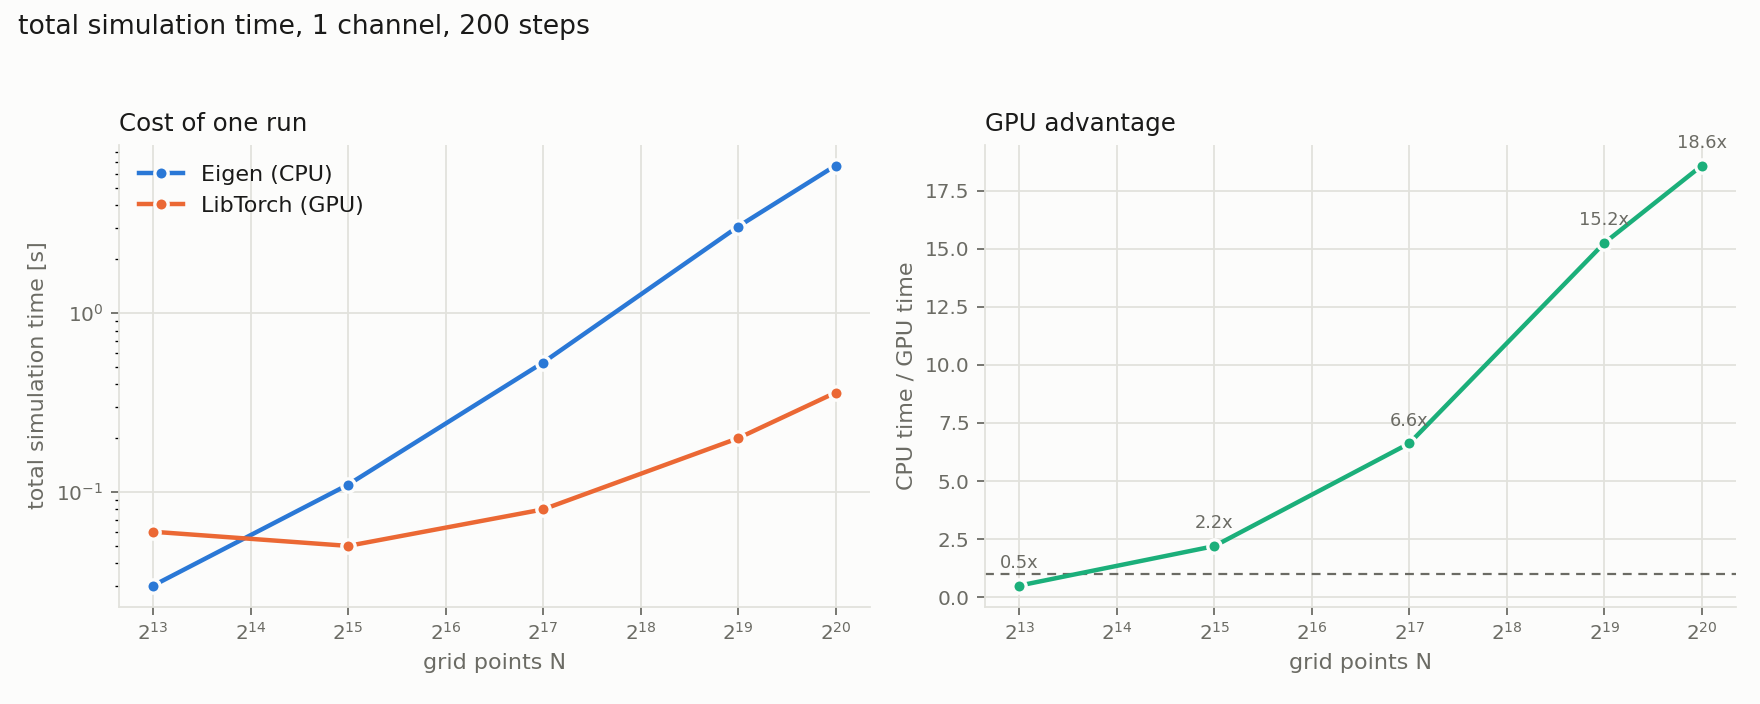
\includegraphics[width=\textwidth]{Figure linear only - Sweeping grid points}
  \caption{Linear-only simulation time and CPU-to-GPU speedup while sweeping the number of
  grid points. The simulation uses one optical channel and 200 propagation steps.}
  \label{fig:linear-grid-sweep}
\end{figure}

The channel-count sweep in \cref{fig:linear-channel-sweep} holds the grid size at 131,072
points and uses 200 propagation steps. The measured GPU speedup ranged from 7.7 for one
channel to 19.9 for 128 channels. This increase is consistent with the GPU using its parallel
compute resources more effectively as more field data is processed. Together, the two sweeps
show that the linear-only GPU implementation benefits from larger grids and more channels,
although the size sweep shows that a GPU is not necessarily faster for small problems.

\begin{figure}
  \centering
  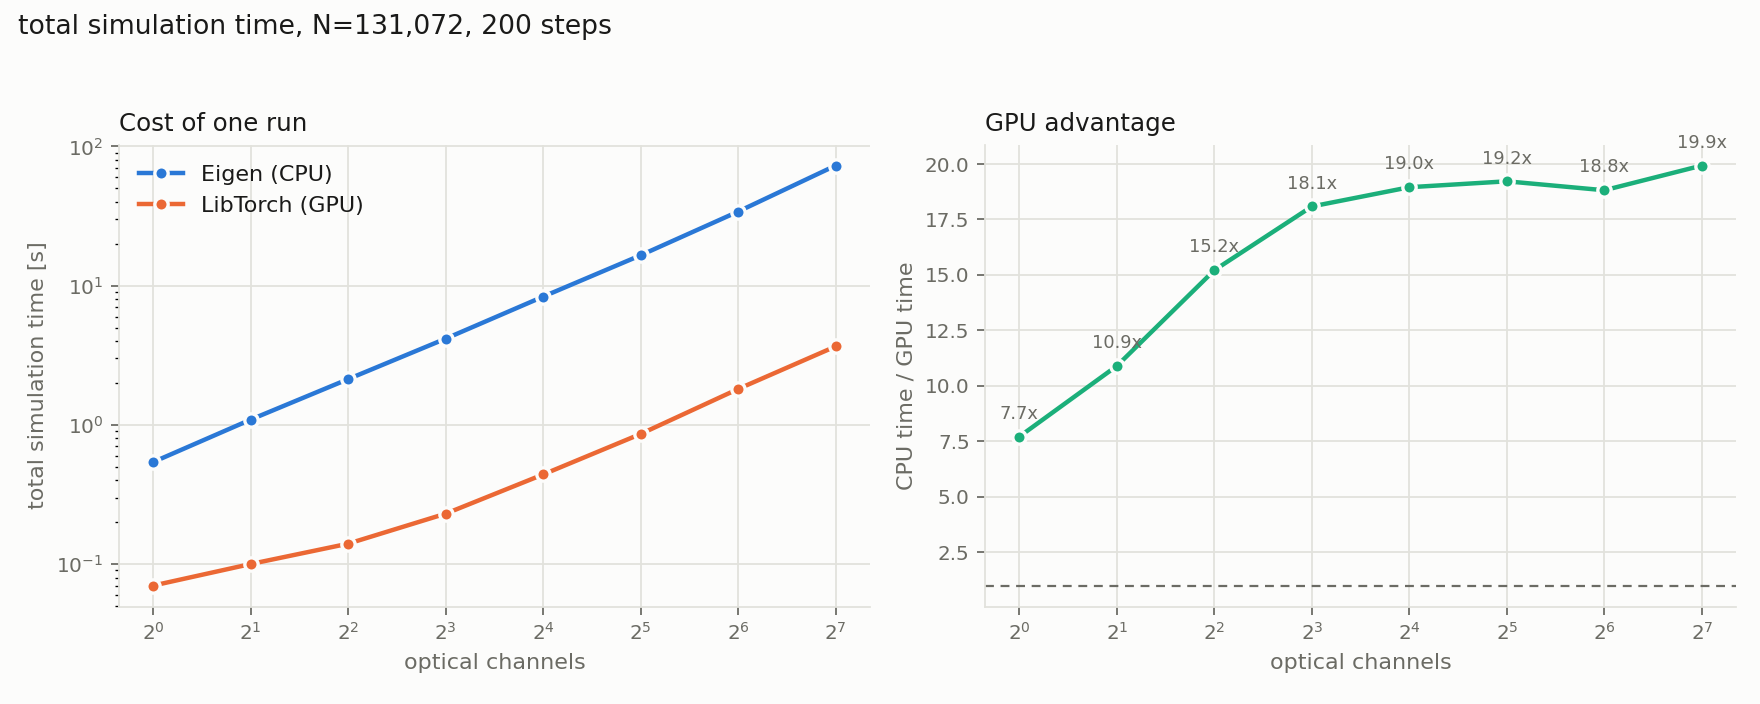
\includegraphics[width=\textwidth]{Figure linear only - sweeping optial channels}
  \caption{Linear-only simulation time and CPU-to-GPU speedup while sweeping the number of
  optical channels. The grid contains 131,072 points and the simulation uses 200 propagation
  steps.}
  \label{fig:linear-channel-sweep}
\end{figure}

Once the nonlinear effects were able to run across both backings through \texttt{FieldData} objects, 
the next experiment enabled nonlinear effects in addition to the linear propagation terms.
This tests whether the performance trend in the linear-only case also holds when the
nonlinear calculation is included, and provides comparison between GPU and CPU speed for the program
as a whole. As mentioned before, grid sizes below $2^{15}$ have their timing dominated by kernel launches
and that explains why they are seen as unusually slow in the right graph of \Cref{fig:four-channel-nonlinear-speed}.

\begin{figure}
  \centering
  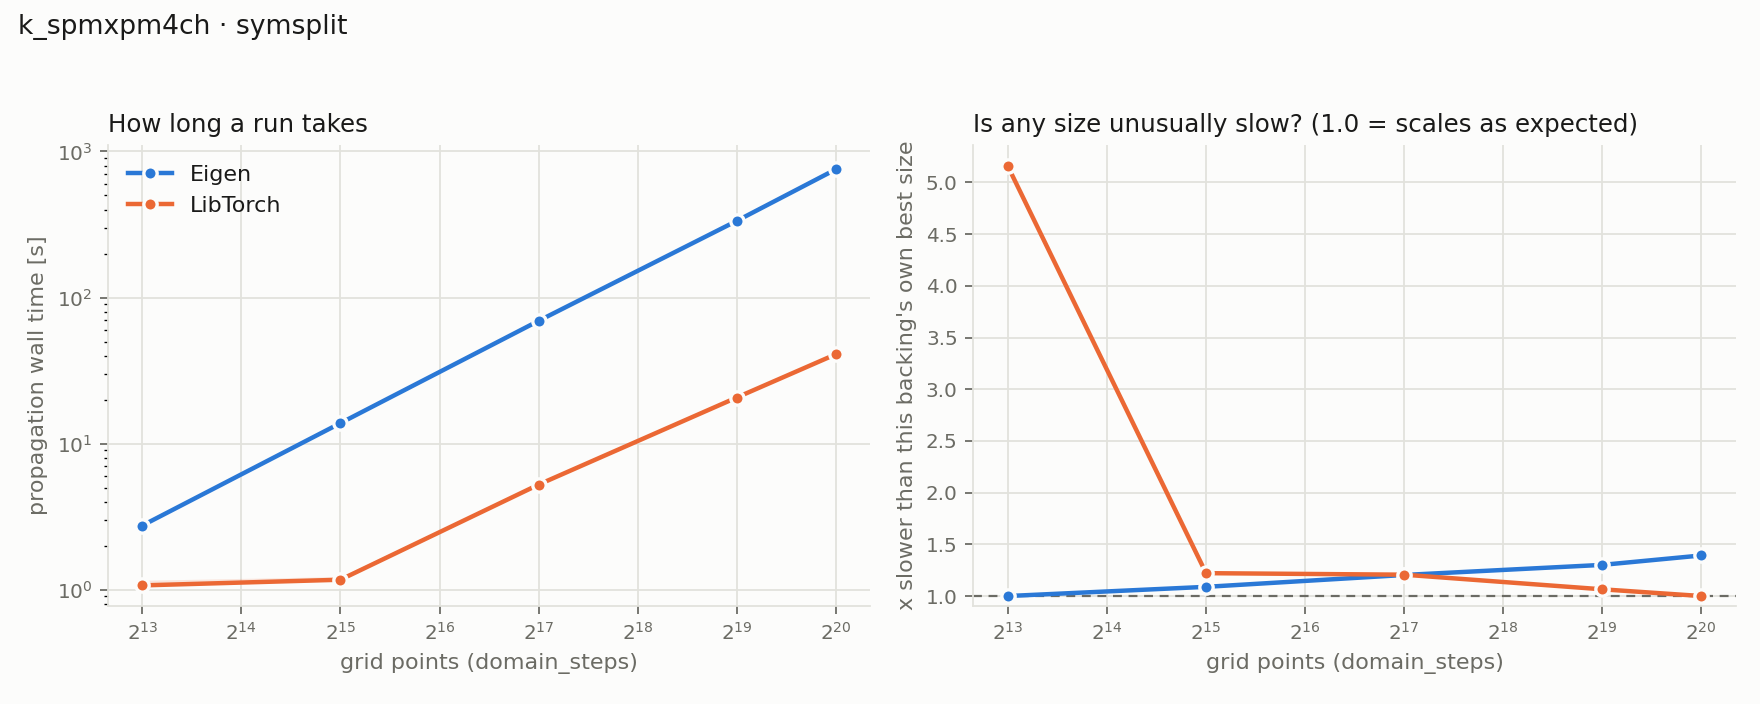
\includegraphics[width=\textwidth]{speed_k_spmxpm4ch_symsplit}
  \caption{Propagation time for the symmetric split-step method with SPM and XPM enabled
  across four optical channels. The left panel shows runtime as grid size increases; the right
  panel compares scaling against each backing's own best result.}
  \label{fig:four-channel-nonlinear-speed}
\end{figure}

\begin{figure}
  \centering
  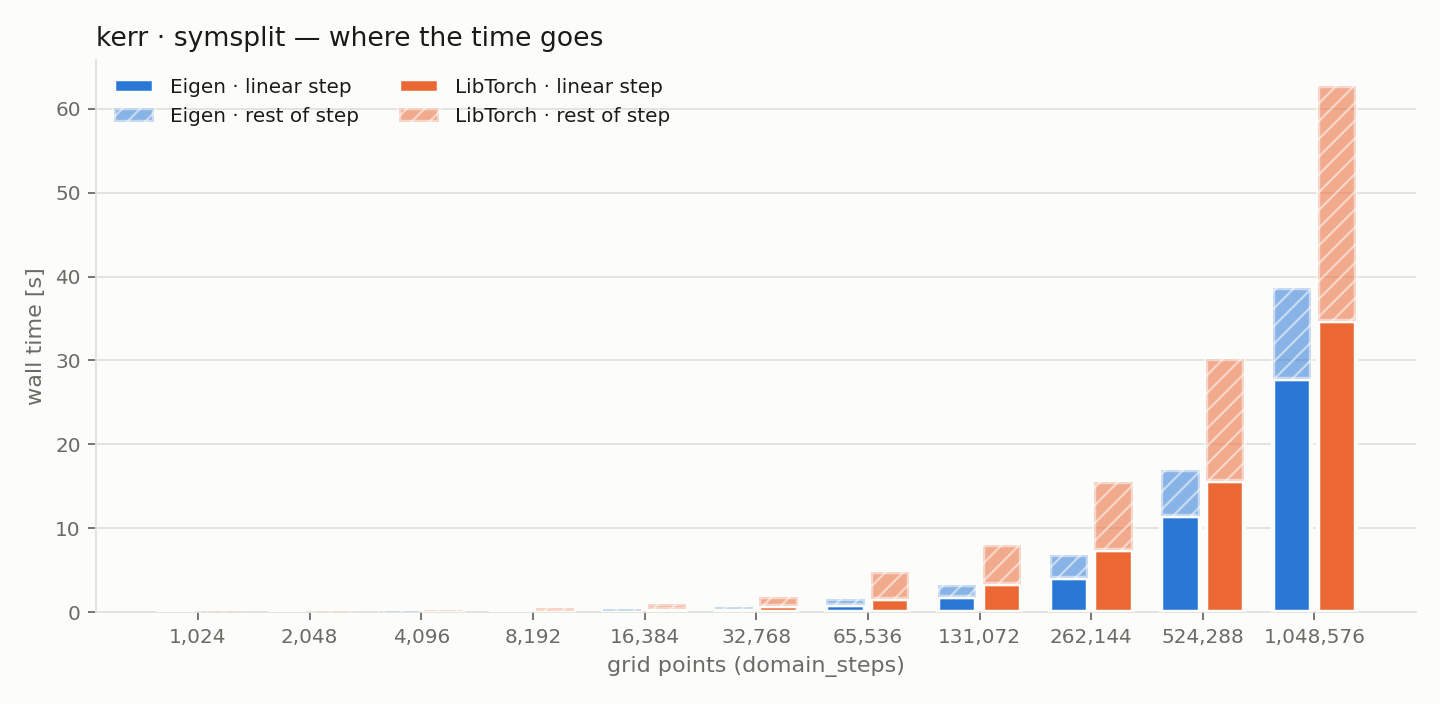
\includegraphics[width=\textwidth]{split_kerr_symsplit}
  \caption{Time spent in the linear step and the remaining work for the Kerr benchmark using
  symmetric split-step. The remaining-work segment includes the nonlinear calculation and
  time outside the measured linear step.}
  \label{fig:kerr-time-split}
\end{figure}

\subsection{Which Parts of the Simulation Take the Most Time?}

The timing breakdown in \Cref{fig:kerr-time-split} compares the linear step with the
remaining work in the simulation. The benchmarks show that the linear part receives a
greater performance improvement from GPU execution than the nonlinear part. This difference
is related to how each part processes the field data (\texttt{svea}). In one SPM-only step,
the nonlinear calculation performs 39 operations and reads or writes \texttt{svea} 84
times. The linear calculation performs 6 operations and reads or writes \texttt{svea} 15
times. The repeated field-data accesses in the nonlinear calculation create more memory
traffic and more intermediate operations, which limits the performance improvement it gets
from the GPU. By comparison, the linear calculation consists largely of FFT operations,
which are well suited to GPU execution. The operation counts provide a simple explanation
for the difference, although the exact performance improvement depends on the hardware and
simulation configuration.

\subsection{Precision and loss effects}

The LibTorch results above use double-precision complex values, matching that of Eigen. 
The FP64 ratio (64 bit floating-point ratio) refers to the throughput ratio of FP64 arithmetic on a GPU
compared to FP32 (32 bit floating-point) arithmetic. Typical consumer GPU cards have an FP64 ratio of 1:64,
meaning that double-precision operations take 64 times as long to be performed.
Common high-end GPUs in HPC can have FP64 ratio as good as 1:2, such as the NVIDIA V100, A100, or H100.
Since double-precision arithmetic can be substantially more expensive on some GPUs than single-precision arithmetic,
a further experiment compares LibTorch performance using 64-bit and 32-bit floating-point
values. The measured runtimes are shown in \Cref{tab:precision-speedup}. Across the tested
grid sizes, single precision was approximately 2.4--2.5 times faster than double precision.
This is however specific to the hardware used; in the following precision comparison, it was a 
Tesla T4 GPU with a FP64 ratio of 1:32.

\begin{table}[H]
  \centering
  \caption{Runtime and speedup for single and double-precision LibTorch simulations on a
  Tesla T4 GPU. The speedup is the double-precision runtime divided by the single-precision
  runtime.}
  \label{tab:precision-speedup}
  \begin{tabular}{rrrrrr}
    \toprule
    $N$ & Double (s) & Float (s) & Speedup & Linear speedup & nonlinear speedup \\
    \midrule
    $2^{20}$ & 9.4 & 3.9 & 2.4$\times$ & 4.1$\times$ & 2.0$\times$ \\
    $2^{21}$ & 18.1 & 7.4 & 2.4$\times$ & 4.1$\times$ & 2.0$\times$ \\
    $2^{22}$ & 36.3 & 14.8 & 2.5$\times$ & 4.2$\times$ & 2.0$\times$ \\
    \bottomrule
  \end{tabular}
\end{table}

The precision comparison introduces a measurable accuracy cost, summarised in
\Cref{tab:precision-error}. The maximum field difference is measured relative to the peak
of the double-precision field. After 1,000 steps the difference remains small, but it grows
substantially after 10,000 steps. The float run also loses energy, with greater loss over the
longer run.

\begin{table}[H]
  \centering
  \caption{Difference and energy change for single-precision LibTorch relative to
  double-precision LibTorch on a Tesla T4, using the symmetric split-step method with
  $N=2^{20}$. The maximum field error is normalised by the peak of the double-precision
  field.}
  \label{tab:precision-error}
  \begin{tabular}{rrr}
    \toprule
    Steps & Maximum field error / peak & Energy change (float) \\
    \midrule
    1,000 & $5.1\times10^{-4}$ & $-0.043\%$ \\
    10,000 & $5.2\times10^{-2}$ & $-0.44\%$ \\
    \bottomrule
  \end{tabular}
\end{table}

An additional dispersion-only test and a direct FFT round-trip test help identify the source
of this energy loss. With nonlinear effects disabled, 1,000 single-precision steps produced
an energy change of $-4.3\times10^{-4}$. Applying 1,000 forward and inverse complex64 FFT
round trips to a field of size $2^{20}$ produced a similar change ($-4.25\times10^{-4}$),
whereas complex128 changed the energy by approximately $4\times10^{-13}$. This indicates
that the observed loss is associated with single-precision FFT round-off in cuFFT rather
than the propagation phase itself. Repeated small downward changes can accumulate over many
steps. The separate error-growth test at 8,192 points shows that the maximum field error
grows approximately linearly with step count when Kerr is disabled, and approximately
quadratically when Kerr is enabled over the measured range. The Kerr-enabled curve follows
the plotted slope-two guide, while the dispersion-only curve grows more slowly. This supports
the interpretation that nonlinear effects compound the numerical differences; these growth
rates describe the tested configuration and range.

\subsection{Summary}

The measurements show that GPU acceleration is most useful once the workload is sufficiently
large. With four channels and SPM/XPM enabled, the GPU also outperformed the CPU for the
tested grid sizes. The timing breakdown shows that the linear and remaining parts of the
simulation contribute differently to total runtime. Although using single precision gave an
approximately 2.4-fold speedup over double precision for the tested grid sizes, the error in
the results makes it unusable past generating a quick answer where exact precision isn't required.
The exact results are specific to the tested hardware and configurations.

\chapter{Discussion}

Overall, the research met its three goals of performance, modularity and portability. The GPU
backing made large simulations substantially faster, custom functions let researchers describe new
pulses and couplings without changing code, and the simulation still builds and runs on machines
without a GPU. Modern C++ features proved useful in getting there. Holding each backing in a
\texttt{std::variant} and dispatching with \texttt{std::visit} kept a single propagation path for both
the CPU and GPU, and meant that a missing implementation was caught by the compiler rather than at
runtime. At the same time, the new code kept to the conventions already in the codebase, such as
configuring components through separate \texttt{setup()} calls. While this departs from standard C++
practice, it is common in scientific computing and kept the new work consistent with how the rest of
the simulation is built.

There are several directions for further work. The single-precision results were promising on speed
but introduced too much error, so more experimentation with 32-bit values, such as keeping only the
FFTs in double precision, could recover much of the speedup without the loss in accuracy. AMD GPUs
are not yet supported, and adding and testing ROCm support would make GPU acceleration available to
more researchers. Adding another \texttt{compute\_backing} type for a library such as SYCL
would give lower-level control over GPU computation, and show that \texttt{FieldData} can support new
data storage.
Finally, the performance improvements were measured on benchmark configurations, and demonstrating them 
on an actual research question would show how much they shorten the time taken to get real results.

% Plan: ~1 page.
\chapter{Conclusion}

This work extended the simulation to support GPU-backed field data and custom pulse
profiles. By adding custom defined functions, users are now able to define their own wave and spatially dependant fields without changing any code.
The research then implemented and proved that GPU acceleration can greatly accelerate simulation, and therefore research speed.
GPU acceleration was seen to have greater benefit as the workload got larger, through increasing grid-size, or number of pulses. 
For small grids, the time taken to launch GPU operations can make the GPU slower than the CPU.
For larger grids and more channels, the GPU was substantially faster, reaching roughly 19x improvements.

The outcome of this research is that the SBS simulation is now capable of utilising the previously
unrealised computational power of the GPU.


\printbibliography[heading=bibintoc,title={Bibliography}]

\appendix
\chapter{Appendix}

\section{Cash--Karp RK5 Stages}
\label{app:rk5}

\begin{equation}
  \label{eq:rk5-stages}
  \begin{aligned}
    A^{(i)} &= U_{h/2}^{\mathcal{D}} A_n, \\
    k_1 &= U_{h/2}^{\mathcal{D}} f(A_n, z_n), \\
    k_2 &= U_{3h/10}^{\mathcal{D}} f\!\left(U_{-3h/10}^{\mathcal{D}}\left[A^{(i)} + \tfrac{h}{5}k_1\right],\, z_n + \tfrac{h}{5}\right), \\
    k_3 &= U_{h/5}^{\mathcal{D}} f\!\left(U_{-h/5}^{\mathcal{D}}\left[A^{(i)} + h\left(\tfrac{3}{40}k_1 + \tfrac{9}{40}k_2\right)\right],\, z_n + \tfrac{3h}{10}\right), \\
    k_4 &= U_{-h/10}^{\mathcal{D}} f\!\left(U_{h/10}^{\mathcal{D}}\left[A^{(i)} + h\left(\tfrac{3}{10}k_1 - \tfrac{9}{10}k_2 + \tfrac{6}{5}k_3\right)\right],\, z_n + \tfrac{3h}{5}\right), \\
    k_5 &= U_{-h/2}^{\mathcal{D}} f\!\left(U_{h/2}^{\mathcal{D}}\left[A^{(i)} + h\left(-\tfrac{11}{54}k_1 + \tfrac{5}{2}k_2 - \tfrac{70}{27}k_3 + \tfrac{35}{27}k_4\right)\right],\, z_n + h\right), \\
    k_6 &= U_{-3h/8}^{\mathcal{D}} f\!\left(U_{3h/8}^{\mathcal{D}}\left[A^{(i)} + h\left(\tfrac{1631}{55296}k_1 + \tfrac{175}{512}k_2 + \tfrac{575}{13824}k_3 + \tfrac{44275}{110592}k_4 + \tfrac{253}{4096}k_5\right)\right],\, z_n + \tfrac{7h}{8}\right).
  \end{aligned}
\end{equation}

\begin{equation}
  \label{eq:rk5-solution}
  A_{n+1}^{(5)} = U_{h/2}^{\mathcal{D}}\left[A^{(i)} + h\left(\tfrac{37}{378}k_1 + \tfrac{250}{621}k_3 + \tfrac{125}{594}k_4 + \tfrac{512}{1771}k_6\right)\right].
\end{equation}

\section{Benchmark Hardware and Results}
\label{app:benchmarks}

\begin{table}[H]
  \centering
  \caption{Hardware used for the benchmarks.}
  \begin{tabular}{lll}
    \toprule
    Benchmarks & CPU & GPU \\
    \midrule
    Linear-only & Xeon Platinum 8259CL (1 core) & Tesla T4 \\
    Kerr & Xeon Platinum 8259CL (1 core) & Tesla T4 \\
    Precision & & Tesla T4 \\
    \bottomrule
  \end{tabular}
\end{table}

\begin{table}[H]
  \centering
  \caption{Linear-only simulation time while sweeping grid size, with one channel and 200 steps.
  Fastest of two repeats.}
  \begin{tabular}{rrrr}
    \toprule
    $N$ & CPU (s) & GPU (s) & Speedup \\
    \midrule
    8,192 & 0.03 & 0.06 & 0.5$\times$ \\
    32,768 & 0.11 & 0.05 & 2.2$\times$ \\
    131,072 & 0.53 & 0.08 & 6.6$\times$ \\
    524,288 & 3.05 & 0.20 & 15.2$\times$ \\
    1,048,576 & 6.69 & 0.36 & 18.6$\times$ \\
    \bottomrule
  \end{tabular}
\end{table}

\begin{table}[H]
  \centering
  \caption{Linear-only simulation time while sweeping the number of channels, with 131,072 grid
  points and 200 steps. Fastest of two repeats.}
  \begin{tabular}{rrrr}
    \toprule
    Channels & CPU (s) & GPU (s) & Speedup \\
    \midrule
    1 & 0.54 & 0.07 & 7.7$\times$ \\
    2 & 1.09 & 0.10 & 10.9$\times$ \\
    4 & 2.13 & 0.14 & 15.2$\times$ \\
    8 & 4.16 & 0.23 & 18.1$\times$ \\
    16 & 8.34 & 0.44 & 19.0$\times$ \\
    32 & 16.53 & 0.86 & 19.2$\times$ \\
    64 & 34.06 & 1.81 & 18.8$\times$ \\
    128 & 72.95 & 3.66 & 19.9$\times$ \\
    \bottomrule
  \end{tabular}
\end{table}

\begin{table}[H]
  \centering
  \caption{Simulation time with SPM and XPM across four channels, 1,000 steps. Median of three repeats.}
  \begin{tabular}{rrrr}
    \toprule
    $N$ & CPU (s) & GPU (s) & Speedup \\
    \midrule
    8,192 & 2.81 & 1.14 & 2.5$\times$ \\
    32,768 & 14.05 & 1.22 & 11.5$\times$ \\
    131,072 & 69.92 & 5.27 & 13.3$\times$ \\
    524,288 & 335.46 & 20.74 & 16.2$\times$ \\
    1,048,576 & 788.75 & 41.28 & 19.1$\times$ \\
    \bottomrule
  \end{tabular}
\end{table}

\begin{table}[H]
  \centering
  \caption{Simulation time with Kerr (SPM) on one channel, 1,000 steps. Median of three repeats.}
  \begin{tabular}{rrrr}
    \toprule
    $N$ & CPU (s) & GPU (s) & Speedup \\
    \midrule
    1,024 & 0.04 & 0.77 & 0.1$\times$ \\
    2,048 & 0.08 & 0.83 & 0.1$\times$ \\
    4,096 & 0.16 & 0.95 & 0.2$\times$ \\
    8,192 & 0.39 & 1.14 & 0.3$\times$ \\
    16,384 & 0.77 & 0.91 & 0.8$\times$ \\
    32,768 & 1.49 & 0.83 & 1.8$\times$ \\
    65,536 & 2.99 & 0.97 & 3.1$\times$ \\
    131,072 & 6.10 & 1.35 & 4.5$\times$ \\
    262,144 & 13.68 & 2.54 & 5.4$\times$ \\
    524,288 & 30.65 & 4.95 & 6.2$\times$ \\
    1,048,576 & 68.56 & 9.55 & 7.2$\times$ \\
    \bottomrule
  \end{tabular}
\end{table}


\end{document}
